\documentclass[a4paper,12pt]{report}
\usepackage[utf8]{inputenc}
\usepackage[T2A]{fontenc}
\usepackage[russian]{babel}
\usepackage{amsmath}
\usepackage{amssymb}
\usepackage{graphicx}
\usepackage{array}
\usepackage{multirow}
\usepackage{booktabs}
\usepackage{geometry}
\usepackage{float}
\usepackage{ulem}
\usepackage{tabularx}
\usepackage{booktabs}
\usepackage{siunitx}
\usepackage{indentfirst}
\usepackage{placeins}
\usepackage{lipsum}
\usepackage{longtable}
\usepackage{csquotes}
\usepackage[style=gost-numeric,sorting=none]{biblatex}
\usepackage{enumitem}




\addbibresource{references.bib}
\usepackage{titlesec}
\titleformat{\chapter}[display]
    {\normalfont\huge\bfseries}
    {\chaptertitlename\ \thechapter}
    {20pt}
    {\Huge}
\usepackage{booktabs}
\usepackage{makecell}
\graphicspath{{Image/}}

\geometry{
    a4paper,
    total={170mm,257mm},
    left=20mm,
    top=20mm,
}

\newcommand{\specialcell}[2][c]{%
    \begin{tabular}[#1]{@{}c@{}}#2\end{tabular}%
}

\usepackage{etoolbox}
\patchcmd{\thebibliography}
  {\chapter*{\bibname}}
  {\section*{\centering СПИСОК ЛИТЕРАТУРЫ}}
  {}{}
\patchcmd{\thebibliography}
  {\addcontentsline{toc}{chapter}{\bibname}}
  {\addcontentsline{toc}{section}{СПИСОК ЛИТЕРАТУРЫ}}
  {}{}


\usepackage{setspace}
\onehalfspacing


\begin{document}





\begin{center}
    \begin{tabular}{cc}

        \specialcell{
\includegraphics[width=0.8in,height=0.9in]{images/BMSTU.jpg}} & 
        \specialcell{
            \textbf{Министерство науки и высшего образования Российской Федерации} \\
            \textbf{Федеральное государственное автономное образовательное учреждение} \\
            \textbf{высшего образования} \\
            \textbf{«Московский государственный технический университет} \\
            \textbf{имени Н. Э. Баумана} \\
            \textbf{(национальный исследовательский университет)»} \\
            \textbf{(МГТУ им. Н. Э. Баумана)}
        } \\
   
    \end{tabular}
\end{center}

\vspace{1cm}

\begin{center}
    \textbf{ФАКУЛЬТЕТ \uline{«СПЕЦИАЛЬНОЕ МАШИНОСТРОЕНИЕ»}}
    
    \textbf{КАФЕДРА \uline{«РАКЕТНЫЕ И ИМПУЛЬСНЫЕ СИСТЕМЫ» (СМ-6)}}
    
    \vspace{1cm}
    
    \textbf{ДОМАШНЕЕ ЗАДАНИЕ}
    
    \vspace{1cm}
    
    ПО ДИСЦИПЛИНЕ:
    
    \vspace{0.5cm}
    
    \begin{tabular}{c}
       
        \specialcell{Проектирование ракетного оружия} \\
        \hline
    \end{tabular}
    
    \vspace{1cm}
    
    НА ТЕМУ:
    
    \vspace{0.5cm}
    
    \begin{tabular}{c}
       
        \specialcell{Массовый анализ AIM-120 AMRAAM} \\
        \hline
    \end{tabular}
    
    \vspace{1cm}

    
    \vspace{1cm}
    

    \begin{tabular}{llp{3cm}l}
       
        Выполнил: студент группы СМ6-62 & 
        (подпись, дата) & 
         & 
        Ерофеев М.В.\\
        \hline
    \end{tabular}
    
    \vspace{1cm}
    
    \begin{tabular}{llp{3cm}l}
    
        Проверил &  (подпись, дата) & & Лаптева Л.А.\\
        \hline
    \end{tabular}
    
    \vspace{6cm}
    
    Москва, 2025 г.
\end{center}
\tableofcontents

\newpage
\chapter*{Принятые сокращения}
\begin{description}[font=\normalfont\itshape] % обычный шрифт + курсив
\item[WDU] — Weapons Detonation Unit (блок подрыва боевой части)
\item[WGU] — Weapons Guidance Unit (блок наведения вооружения)
\item[WPU] — Weapons Propulsion Unit (двигательный отсек вооружения)
\item[ICPU] — Integrated Control and Power Unit (встроенный блок управления и питания)
\item[РДТТ] — ракетный двигатель твердого топлива
\item[БЧ] — боевая часть
\end{description}


\newpage
\chapter{Краткие сведения о прототипе}
\section{Обзор прототипа}
Ракета AIM-120A AMRAAM (Advanced Medium-Range Air-to-Air Missile –усовершенствованная ракета класса "воздух-воздух"  средней дальности) выполнена по нормальной аэродинамической схеме с «Х» – образным расположением консолей крыла и рулей.

\begin{figure}[h!]
\centering
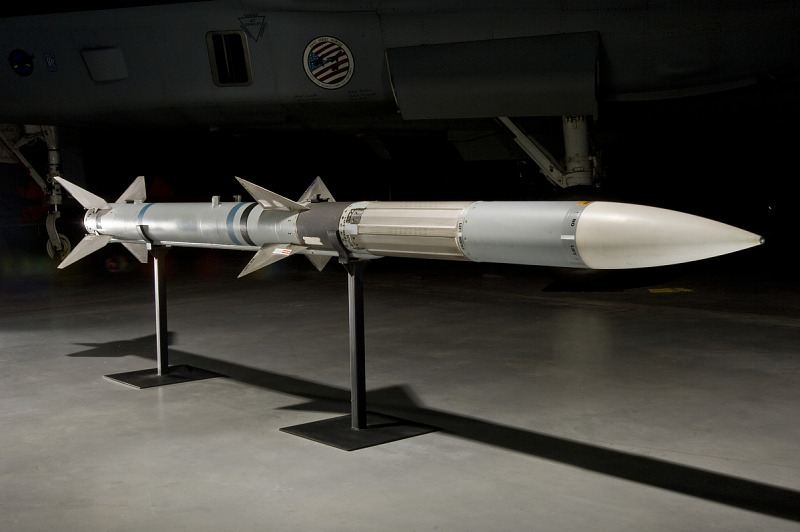
\includegraphics[width=0.7\textheight]{images/1.jpg}
\caption{Ракета AIM-120 AMRAAM}
\label{AIM-120}
\end{figure}

\newpage
\section{Внешнее описание}
Ракета цилиндрическая, длинная, со стреловидным обтекателем.
Носовая часть имеет длину 18.5 дюймов и окрашена в белый цвет. Далее расположена секция батарей серого цвета длиной 17.5 дюймов. Имеется желтая и чёрная полоса с надписью «Осторожно — Используйте защитный чехол для обтекателя».
Следом идет неокрашенная серая секция управления (WCU) длиной 18.75 дюймов. За ней расположена секция БЧ (WDU), длиной 9.5 дюймов, темно-серого цвета.
Эта секция снизу переходит в более светло-серую секцию РДТТ (WPU) длиной 74.75 дюймов. На ней в верхней части расположена черная и синяя полосы, обозначающие, что это учебный снаряд.
За секцией РДТТ находится секция управления рулями длиной 14.75 дюймов. Рули длинные, частично треугольной формы с прямым краем сверху. На них наклеены красно-белые полосы и нанесены номера.
Передние крылья также имеют наклейки и номера. Они алюминиевые, треугольной формы. На ракете присутствуют ушки для крепления к пилону.


\begin{figure}[h!]
\centering
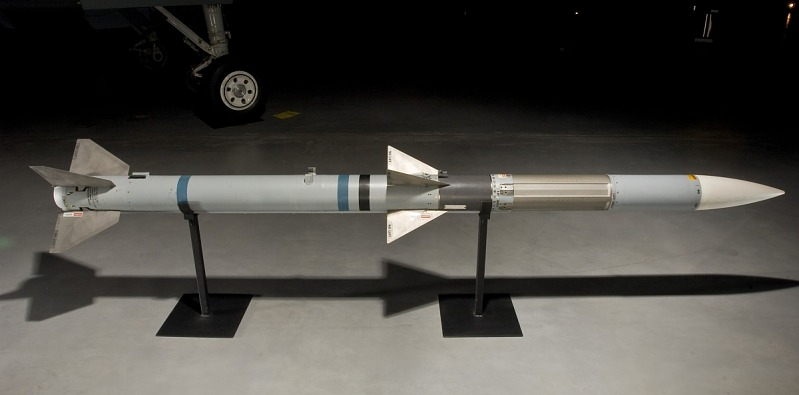
\includegraphics[width=0.55\textheight]{images/2.jpg}
\caption{Ракета AIM-120 AMRAAM}
\label{AIM-120}
\end{figure}

\begin{figure}[h!]
\centering
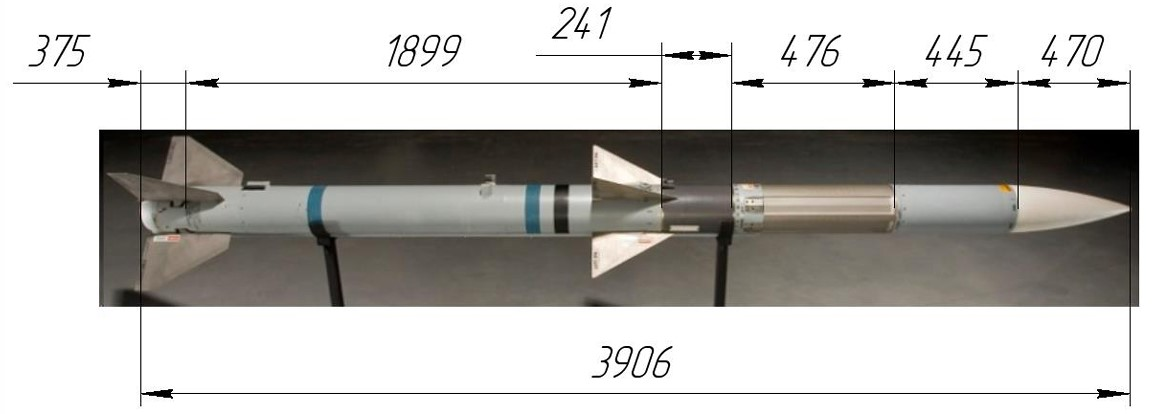
\includegraphics[width=0.65\textheight]{images/3.jpg}
\caption{Размеры отсеков в миллиметрах}
\label{AIM-120}
\end{figure}

\newpage
\section{Внутрення компоновка}
На рисунке 1.4 представлена внутрення компоновка AIM-120, перевод названий модулей дан ниже.

\begin{figure}[h!]
\centering
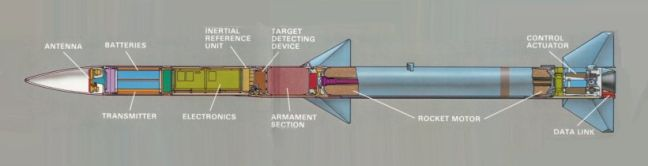
\includegraphics[width=0.7\textheight]{images/4.jpg}
\caption{Компоновка ракеты AIM-120}
\label{AIM-120}
\end{figure}

\begin{description}[font=\normalfont\itshape] % обычный шрифт + курсив
\item[Antenna] — антенна головки самонаведения
\item[(Thermal) batteries] — пиротехнические баратареи, часть ICPU
\item[Transmitter] — передатчик, излучатель
\item[Electronics] — электроника 
\item[Inertial Reference Unit (IRA)] — инерциальная система наведения 
\item[Target Detecting Device (TDD)] — устройство обнаружения цели
\item[Armament Section] — боевая часть 
\item[Rocket Motor] — РДТТ
\item[Contol Actuator] — рулевая машинка
\item[Data Link] — канал передачи данных 
\end{description}

Ниже на рисунке 1.5 представлено разбиение компоновки ракеты на 4 отсека в соответсвии с требованиями ДЗ.

\begin{figure}[H]
\centering
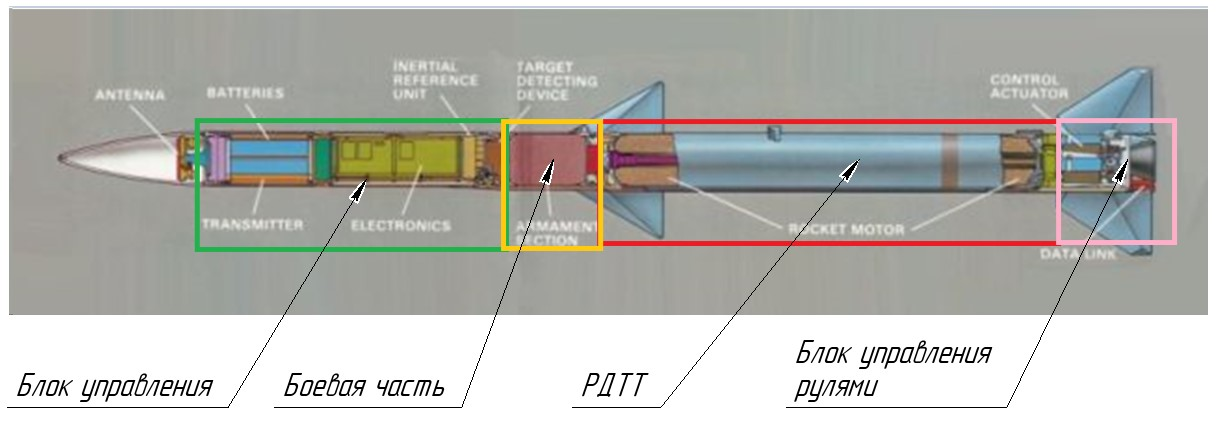
\includegraphics[width=0.65\textheight]{images/5.jpg}
\caption{Схема разбиения компоновки ракеты}
\label{AIM-120}
\end{figure}

\chapter{Массовый анализ}
\section{Расчёт масс отсеков из размеров ракеты}
Расчёт основан на имеющихся данных о массе ракеты, её боевой части из открытых источников. Масса РДТТ бралась из ДЗ по ПрРО предыдущего семестра. Масса остальных отсеков будет найдена
с помощью установленных зависимостей из [1].

Общая масса ракеты — 161.5 кг, масса БЧ — 22 кг. Масса РДТТ — 54.33 кг.

\begin{tabular}{ll}
    \textbf{Дальность}: & 35 морских миль (64.82 км); \\
    \textbf{Скорость}: & 4 Маха; \\
    \textbf{Максимальная длина}: & 12.81 футов (3.9 м); \\
    \textbf{Калибр}: & 0.58 футов (0.178 м).
\end{tabular}

Первый шаг заключается в расчете общего объема ракеты на основе
указанных выше длины и калибра по следующей формуле

\[V = \frac{\pi D^2 L}{4} = \frac{\pi (0.58)^2 \cdot 12.81}{4} = \SI{3.38}{ft^3}\]

Для того что
бы получить оценочное значение массы, выбирается уравнение 4 из анализа общей массы УРВВ:
\[W = 142.2\cdot(V)^{0.74},\]
\[W = 142.2 \cdot (3.38)^{0.74} = 350.18\text{ фунтов}(158.83\text{ кг})\] 

Данное оценочное значение может быть проверено с помощью уравнения 17, разработанного для ракет средней дальности:

\[ W = 177.5\cdot(V)^{0.73} \]

\[ W = 177.5\cdot(3.38)^{0.73} = 431.82 \text{ фунтов}(195.87\text{ кг}) \]

 Поскольку полученные значения отличаются, проводится сравнение со
ответствия для каждого из них. Выбирается уравнение 4, по причине более высокого значения R — квадрат. Таким образом, значение массы при
 начальной оценке равно 350.18 фунтов (158.83 кг). Следовательно, при из
вестных массе и объеме общая плотность изделия может быть рассчитана
 с помощью уравнений:30,


\[ \textit{DENS} = \frac{\textit{W}}{\textit{V}} \]

\[ \textit{DENS} = 103.6 \, \frac{\text{фунтов}}{\text{фут}^3} . \]

Затем вводятся уравнения, разработанные для масс отсеков с параметрами, которые были выведены и оценены. Во-первых, масса отсека ДУ
может быть оценена с помощью уравнения 77:

\[ \textit{PWt} = -284.9 + 633.6(D) - 0.105(W) + 0.949(\textit{DENS}); \]
\[ \textit{PWt} = -284.9 + 633.6(0.58) - 0.105(350.18) + 0.949(103.6) = 169.75 \text{ фунтов}(76.99 \text{ кг})\]


Данное значение проверяется уравнением 82:

\[ \textit{PWt} = 1548.0 - 43.7(L) - 1253.9(D) + 1.4(W) - 6.0(\textit{DENS}); \]
\[ \textit{PWt} = 1548.0 - 43.7(12.81) - 1253.9(0.58) + 1.4(350.18) - 6.0(103.6) = 129.593 \text{ фунтов}(58.78 \text{ кг}) \]

Эти уравнения дали большое расхождение. Так как уравнение
82 имеет лучшее соответствие значению массы РДТТ из ДЗ, для определения
массы отсека ДУ будет использоваться значение 129.593 фунтов (58.78 кг).

 Масса и размер отсека наведения и управления будут оценены анало
гичным образом: оценка массы отсека будет получена из уравнения 85:

\[ GCWt = 117.6(D) + 1.6(R) - 0.14(\textit{DENS}); \]
\[ GCWt = 117.6(0.58) + 1.6(35) - 0.14(103.6) = 109.74 \text{ фунтов}( 49.77\text{ кг}) \]


Теперь определим массу и размеры отсека боевой части. Для оценки массы используем уравнение 93:

\[ WHWt = 0.1(DENS) - 0.2(R) + 0.2(W) - 2.4(L); \]
\[ WHWt = 0.1(103.6) - 0.2(35) + 0.2(350.18) - 2.4(12.81) = 42.652 \text{ фунтов}( 19.34\text{ кг}) \]


Масса рулевого отсека будет рассчитана из общей массы ракеты:

\[
ROW = Wt - GCWt - PWt - WHWt = 350.18 - 109.74 - 129.59 - 42.65 = 68.2 \, \text{ фунтов}( 30.93\text{ кг})
\]

Итого: 

\begin{table}[H]
\centering
\begin{tabular}{|c|c|c|}
\hline
\textbf{Отсек} & \textbf{Имеющиеся данные, кг} & \textbf{Регрессионный анализ, кг} \\
\hline
БЧ & 22 & 19.34 \\
\hline
РДТТ & 54.33 & 58.78 \\
\hline
Блок управления & ??? & 49.77 \\
\hline
Рулевой отсек & ??? & 30.93 \\
\hline
Общая масса ракеты & 161.5 & 158.8 \\
\hline
\end{tabular}
\caption{Результаты анализа}
\label{tab:three_columns}
\end{table}

Примем реальное значение боевой части, массу РДТТ  возьмем из ДЗ, а массу блока управления и рулевого отсека возьмём из регрессонного анализа. Тогда:
\begin{table}[H]
\centering
\begin{tabular}{|c|c|}
\hline
\textbf{Отсек} & \textbf{Масса отсека, кг} \\
\hline
БЧ & 22 \\
\hline
РДТТ & 54.33\\
\hline
Блок управления & 49.77\\
\hline
Рулевой отсек & 30.93 \\
\hline
Общая масса ракеты & 157.03 \\
\hline
\end{tabular}
\caption{Принятые массы}
\label{tab:three_columns}
\end{table}

\section{Расчёт плотностей отсеков}

Расчёт будет производиться по формуле:

\[ \rho = \frac{m}{V}, \quad \left[\frac{\text{кг}}{\text{м}^3}\right] \]

Но сначала необходимо высчитать объемы отсеков по формуле: 

\[V = \frac{\pi D^2 L}{4} \]

1) Объём боевой части:

\[V_{\text{БЧ}} = \frac{\pi (0.178)^2 \cdot 0.241}{4} = 0.0059{\text{ м}^3} \]

2) Объём РДТТ:

\[V_{\text{РДТТ}} = \frac{\pi (0.178)^2 \cdot 1.9}{4} = 0.047{\text{ м}^3} \]

3) Объём блока управления:

\[V_{\text{БУ}} = \frac{\pi (0.178)^2 \cdot 0.921}{4} = 0.0229{\text{ м}^3} \]

4) Объём рулевого отсека(блока рулей):

\[V_{\text{БР}} = \frac{\pi (0.178)^2 \cdot 0.375}{4} = 0.0093{\text{ м}^3} \]

Плотности:

1) Плотность боевой части:

\[ \rho_{\text{БЧ}} = \frac{22}{0.0059} = 3728.81 \quad \left[\frac{\text{кг}}{\text{м}^3}\right]\]

2) Плотность РДТТ:

\[ \rho_{\text{РДТТ}} = \frac{54.33}{0.047} = 1155.95 \quad \left[\frac{\text{кг}}{\text{м}^3}\right]\]

3) Плотность блока управления:

\[ \rho_{\text{БУ}} = \frac{49.77}{0.0299} = 1664.54 \quad \left[\frac{\text{кг}}{\text{м}^3}\right]\]

4) Плотность рулевого отсека(блока рулей):

\[ \rho_{\text{БР}} = \frac{30.93}{0.0093} = 3325.80 \quad \left[\frac{\text{кг}}{\text{м}^3}\right]\]

Перед тем как перейти к построению 3D модели необходимо найти массу двигательной установки.Для этого воспользуемся коэффициентом конструктивно-массового совершенства $\beta$.
Для ракеты AIM-120 он равен $\beta$ = 1.2. Найдем начальную массу топлива и вычтем её из общей массы РДТТ:

\[ m_{\text{т0}} = \frac{54.33}{1.2}=45.275 {\text{ кг}}\]

Найдем массу двигательной установки:

\[ m_{\text{ДУ}} = 54.33-45.275=9.055 {\text{ кг}}\]

Плотность отсека РДТТ после прогорания топлива:

\[ \rho_{\text{РДТТ1}} = \frac{9.055}{0.047} = 192.6595 \quad \left[\frac{\text{кг}}{\text{м}^3}\right]\]

\chapter{Расчёт центра масс}

\section{Построение 3D модели}

Для построения 3D модели используем САПР Компас 3D. Каждый отсек ракеты мо-
делируем отдельно и указываем его плотность и массу. Создаём сборку (рис. 3.1) с полной
массой топлива и без топлива и смотрим на свойства модели.

\begin{figure}[h]
\centering
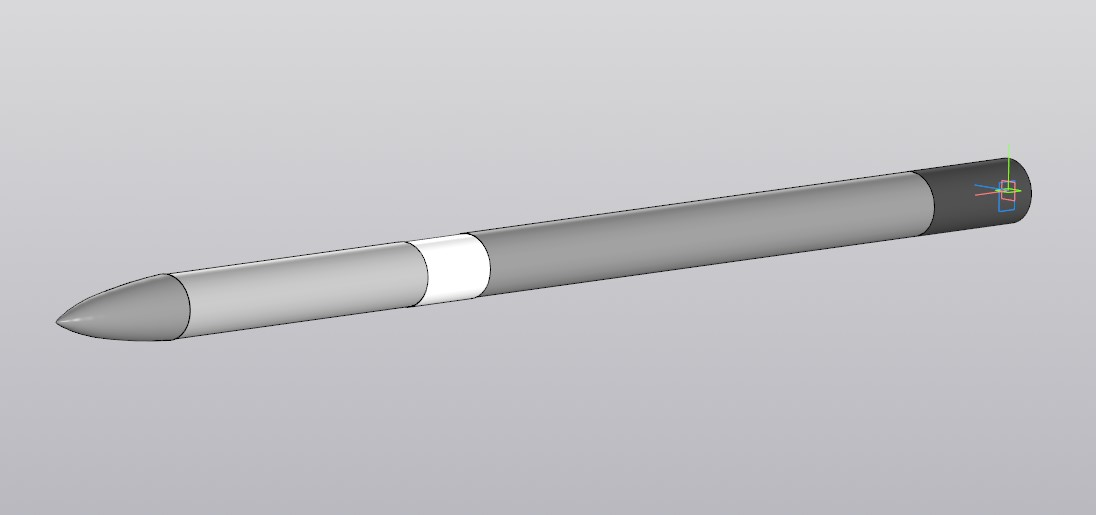
\includegraphics[width=0.65\textheight]{images/6.jpg}
\caption{Сборка ракеты в САПР Компас 3D}
\label{AIM-120}
\end{figure}

\section{Вычисление центра масс}

Вычисление проводилось с помощью САПР Компас 3D. Результаты приведены в таблице 3.1.

\begin{table}[h]
\centering
\begin{tabular}{|p{0.2\textwidth}|p{0.2\textwidth}|p{0.2\textwidth}|p{0.2\textwidth}|}
\hline
\textbf{Состояние бака} & \textbf{x, мм} & \textbf{y, мм} & \textbf{z, мм} \\
\hline
Полный & 0 & 0 & 1677.67 \\
\hline
Пустой & 0 & 0 & 1837.40 \\
\hline
\end{tabular}
\caption{Координаты центра масс при различных состояниях бака}
\label{tab:four_columns}
\end{table}

Зависимость положения центра тяжести от времени z(t) будет выглядеть так: 

\[z = 9.983\cdot t + 1677.67 \]

Стоить отметить, что время горения шашки твердового топлива составляет 16 секунд (данные из ДЗ по ПрРО за прошлый семестр).
\newpage
\begin{thebibliography}{9}

\bibitem{} \textbf{Nowell J. B. Jr.} Missile Total and Subsection Weight and Size. June 1992.

\bibitem{} \textbf{NAVY TRAINING SYSTEM PLAN} AIM-120 ADVANCED MEDIUM RANGE
 AIR-TO-AIR MISSILE. June 1998.

\end{thebibliography}

\end{document}